\documentclass[a4paper]{article}

\usepackage[english]{babel}
\usepackage[utf8]{inputenc}
\usepackage{amsmath}
\usepackage{graphicx}
\usepackage{listings}
\usepackage{algorithmic}
\usepackage[ruled]{algorithm2e} % For algorithms
\usepackage[colorinlistoftodos]{todonotes}

\title{High Performance Computing and Big Data - Cloud computing}

\author{Federico Tavella, Student number 11343605}

\date{\today}

\begin{document}
\maketitle

\section{Exercise 1}

%Explain Oliver what your idea is: tell him which features of the HPC Cloud you are going to use to tackle his problem. Tell him how beautiful your answer is because... do you need to change the montecarlo program?

In order to tackle this problem, we can use the HPC Cloud to allocate multiple virtual machines, each of which will compute part of the "pie".

For example, let's consider a scenario where Oliver is the chief cook and he has $N$ cook assistants. In this scenario, we can cook the pie by assembling $N$ small pies cooked by different chefs. However, the assistants are not self-aware of how to cook the pie, so they need to follow the intructions given by the chief. At this point, Oliver can send the receipt (i.e., the \texttt{montecarlo} program) to each assistant and order them to cook part of the pie. Moreover, Oliver himself could partecipate to the preparation of the pie by preparing his part, reducing the number of assistants from $N$ to $N-1$. Finally, all the small pies can be combined to compose the final pie.

We can see how this approach does not need to change the montecarlo program, but it focuses on distributing the amount of work among different workers (i.e., virtual machines).

\section{Exercise 2}

%Oliver’s recipe is missing pictures. Draw a sketch that Oliver can keep next to his recipe forever, that illustrates what you came up with in the previous exercise.

\begin{figure}[htbp]
\centering
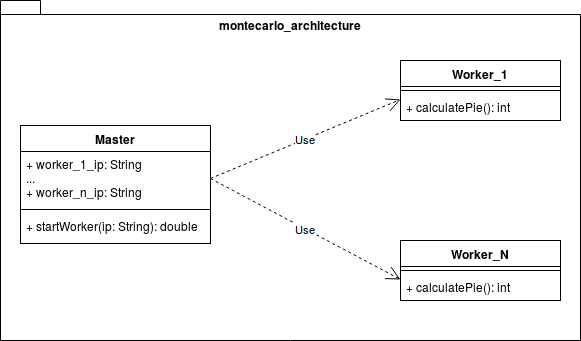
\includegraphics[width=\textwidth]{res/montecarlo.png}
\caption{UML diagram of the problem.}
\label{fig:montecarlo}
\end{figure}

In Figure~\ref{fig:montecarlo}, each partecipant is represented by one class. In our scenario, Oliver is the master who is telling to the other assistants (i.e., workers) how to cook the pie. Each cook is one different virtual machine inside the same network, with an internal IP associated. Since the master knows every IP of the workers, he can send the task to them.

\section{Exercise 3}

%Sketch in pseudocode (https://en.wikipedia.org/wiki/Pseudocode) what you think the programs look like: the master and the worker.
Algorithm~\ref{alg:master} explains how the program for the master looks like. Basically, the master divides the number of points by the number of worker - thus $N'$ - to distribute equally the task among the worker (obviously, if $N$ is not a multiple of $W$ there will be a worker with more points to compute). This suddivision is implicitly done with \texttt{OpenMP} or \texttt{MPI}. Each worker, illustrated with Algorithm~\ref{alg:worker}, computes the number of points $M'$ contained in the circle of radius $R$. This part is executed parallely among all worker. Consequently, the number of points inside the circle is calculated as the sum of all the values provided by the workers and, finally, we can compute an approximation of $\pi$.

\begin{algorithm}[htbp]
%\SetAlgoNoLine
\KwIn{N amount of points, R radius, W number of workers}
\KwOut{An approximation of $\pi$}
$N' \leftarrow N/W$\;
\ForAll{$worker$ in $W$}{
	\textit{calculate M' with N' points using worker}\;
	\textit{store M'}
}
\textit{Wait last worker to finish}\;
$M \leftarrow \sum(M')$\;
$\pi \leftarrow 4 \cdot M/N$\;
\caption{Pseudocode for the master.}
\label{alg:master}
\end{algorithm}

\begin{algorithm}[htbp]
%\SetAlgoNoLine
\KwIn{N' amount of points, R radius}
\KwOut{M' number of points inside the circle of radius R}
$M' \leftarrow 0$\;
\ForAll{$point$ \textbf{in} $N'$}{
	\If{$isInside(point, circle(R)) = True$}{
		$M' \leftarrow M' + 1$\;
	}
}
\caption{Pseudocode for the worker.}
\label{alg:worker}
\end{algorithm}

\section{Exercise 4}

Firstly, we need to create the virtual machine representing the master. We can use the template from the \texttt{MPI} extra exercise, tweaking the values for this problem (e.g., reducing the number of cores to 1 and making the image non-persistent). Once the master has been created, we need to configure it for SSH communication and also with the \texttt{makeme\_master.sh} script. Secondly, we need to create one virtual machine for each worker. Even in this case, we can re-use the \texttt{MPI} template. For each worker node, we need to set a password and to configure it using the \texttt{makeme\_worker.sh} script, in order to indicate to the node who is the master.

\section{Exercise 5}

% Having to create all workers by hand is very tedious. You are so happy that you can show Oliver how to let the master create the workers on demand!!! Thus, for a solution where the master will create the workers on demand (the master now receives the amount of workers, W, as an extra parameter):   

\subsection{Extra components}

%a) What extra components from the HPC Cloud do you need to let the master create the workers?
In order to provide the possibility for the master to create the workers, we need to integrate the \texttt{XML-RPC} API in our project. This allow us to create/deploy/terminate \textbf{programmatically} virtual machines.

\subsection{Pseudocode}

%b) Do the same as in exercise 3: write pseudocode for what the master looks like. Does the worker change? Think of releasing resources when the computation is finished!

In Algorithm~\ref{alg:master_2} we can see how the pseudocode for the master changes. In fact, now the master has the responsability to allocate and deallocate virtual machines corresponding to the workers. However, in this way we have a more efficient consumption of resource: once a worker complete its task, we can release the resources that otherwise would be held until we release them throught the UI.

\begin{algorithm}[htbp]
%\SetAlgoNoLine
\KwIn{N amount of points, R radius, W number of workers}
\KwOut{An approximation of $\pi$}
\textit{//T is the template used for the workers}\;
\ForAll{$worker$ in $W$}{
	$worker_{id} \leftarrow allocateVM(worker,T)$\;
	$deployVM(worker_{id})$\;
	\textit{calculate M' with N' points using worker}\;
	\textit{store M'}\;
	$terminateVM(worker_{id})$\;
}
$M \leftarrow \sum(M')$\;
$\pi \leftarrow 4 \cdot M/N$\;
\caption{Pseudocode for the master.}
\label{alg:master_2}
\end{algorithm}

\subsection{UI relevant steps}

%c) Do the same as in exercise 4: write the relevant steps that you must follow in the UI to run the new version of the master (yes, assume again that you get a program with this version of the master’s work) and workers; again, 1 master and 3 workers

Using \text{XML-RPC}, we can avoid to use the UI to create the virtual machines. Thus, we can create the master and the workers programmatically. Obviously, we need a template to do so, but that could also be created without the UI.

\end{document}